%HW05.tex
%Fifth Homework -- Math 629 
%
%  The percent sign is a comment character
%
%%%%%%%%%%%%%%%%%%%%%%%%%%%%%%%%%%%%%%%%%%%%%%%%%%%%%%%%%%%%%%%%%%%%%%%%%%%%%%%%%%
%
%   Look these up on line.  The first sets the type of document, and the next are for mathematics symbols, graphics and color
%
\documentclass[12pt]{article}
\usepackage{amssymb,amsmath}
\usepackage{graphicx}
\usepackage[usenames,dvipsnames,svgnames,table]{xcolor}
\usepackage{multirow}   % This is for more control over tables
%%%%%%%%%%%%%%%%%%%%%%%%%%%%%%%%  Layout     %%%%%%%%%%%%%%%%%%%%%%%%%%%%%%%%%%%%%%
\usepackage{vmargin}
\setpapersize{USletter}
\setmargrb{2cm}{1cm}{2cm}{1cm} % --- sets all four margins LTRB


%%%%%%%%%%%%%%%%%%%%%%%%%%%%%%%%%%%%%%%%%%%%%%%%%%%%%%%%%%%%%%%%%%%%%%%%%%%%%%%%%
\begin{document}
\LARGE 
\noindent
{\color{Maroon}History of Mathematics \hfill Math 629}\vspace{2pt}\\
\large
Fifth Homework: \hfill 14 February 2024\\
Due Monday 19 February 2024.
\normalsize\vspace{10pt}

To hand in: We are using Gradescope for homework submission.


\begin{enumerate}

\item  {[25]}
  Exercises 6.2.1 --- 6.2.3 from Stillwell.
  The three steps each explained; for the first subtract the first equation from the second, two times.
  Here is a picture of the two curves:
  \[  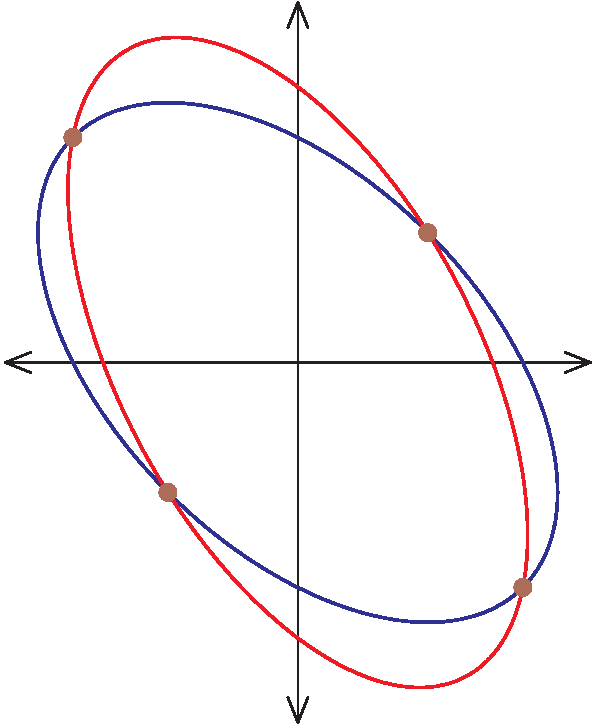
\includegraphics[height=120pt]{TwoEllipses}  \]

   \item  {[15]}
     Exercise  6.5.3 from Stillwell.
    Also find the other two solutions (this may require reading my notes on cubics.)

  \item  {[15]}
    Here is another cubic to solve completely: % $x^3=7x+6$.  That one is too hard
    $4x^3+5x=3$.
 
  \item  {[25]}
    Exercises 6.7.1, 6.7.2, and 6.7.3 in Stillwell. These should be relatively short.

  \item  {[20]}
    Cardano led an interesting life.
    Look up some material on the web (two sources besides our book) and write something about his life, both mathematical
    and otherwise.
    Probably two paragraphs, and try to include some story that is not in Stillwell's potted biography. 
\end{enumerate}

\end{document}
%%%%%%%%%%%%%%%%%%%%%%%%%%%%%%%%%%%%%%%%%%%%%%%%%%%%%%%%%%%%%%%%%%%%%%%%%%%%%%%%%
